\documentclass[12pt]{article}

\usepackage[margin=1in]{geometry} 
\usepackage{amsmath,amsthm,amssymb,mathrsfs,float,fancyhdr,bbm,hyperref,enumerate,float,nicefrac,breqn}

\usepackage[dvipsnames]{xcolor}
\usepackage{graphicx} 

\newcommand{\N}{\mathbb{N}}
\newcommand{\Z}{\mathbb{Z}}
\newcommand{\R}{\mathbb{R}}
\newcommand{\C}{\mathbb{C}}
\newcommand{\B}{\mathbb{B}}
\newcommand{\Q}{\mathbb{Q}}
\newcommand{\F}{\mathscr{F}}
\newcommand{\E}{\mathbb{E}}
\newcommand{\PP}{\mathbb{P}}
\newcommand{\Var}{\mathrm{Var}}
\newcommand{\Cov}{\mathrm{Cov}}

\newtheorem{problem}{Problem}
\newtheorem{theorem}{Theorem}[section]
\newtheorem{axiom}{Axiom}[section]
\newtheorem{lemma}[theorem]{Lemma}
\newtheorem{proposition}[theorem]{Proposition}
\newtheorem{corollary}[theorem]{Corollary}
\renewcommand{\qedsymbol}{$\blacksquare$}
\newenvironment{definition}[1][Definition]{\begin{trivlist}
\item[\hskip \labelsep {\bfseries #1}]}{\end{trivlist}}

\hypersetup{
    colorlinks=true,
    linkcolor=blue,
    filecolor=magenta,      
    urlcolor=Green,
}


%%%this package allows nice indention for enumerate
\usepackage{enumitem}
\setlist{  
  listparindent=\parindent,
  parsep=0pt,
}
%\begin{enumerate}[label=(\alph*)]
%\begin{enumerate}[label=(\roman*)]
%http://www.texnia.com/archive/enumitem.pdf


\renewcommand{\arraystretch}{1.1} %set the distance across lines in table



%%%http://detexify.kirelabs.org/classify.html 
%%%find unknown symbols by drawing
%%%\mathbbm{1} for indicator function 

\usepackage{mathtools}
%mathtools extends amsmath with {dcases} for {cases} -- prettier

\DeclarePairedDelimiter\floor{\lfloor}{\rfloor} %floor function 

%\usepackage[nomarkers,figuresonly]{endfloat} %put all figures at the end
%\renewcommand{\efloatseparator}{\mbox{}} %if one wants to put multiple figures in one page

\usepackage{pdflscape}
\usepackage{booktabs}
\usepackage{multirow} 
\usepackage{bm}
\usepackage{threeparttable}

\begin{document}
\title{Replication of ``Resurrecting the (C)CAPM: A Cross-Sectional Test When Risk Premia Are Time-Varying" \\by  Martin Lettau and Sydney Ludvigson}
\author{Huangyu Chen}
\maketitle

\begin{abstract}
 I replicate the original paper and extend it to include most recent data,  from 1973:Q3 to 2015:Q3. The conclusions remain valid overall, the average pricing errors with new data increase for all models and goodness of fit decreases. Moreover, the average realized returns seem to be systematically bigger than all the models' predictions, this implies that all the models fail to incorporate certain (macro) risk factors. This might be related to the Dot-com Bubble and Financial Crisis which were not included in the original data set.  Last, joint alpha test of zero pricing error has poor small sample property. Shanken's correction for time-series correlation in errors seems to be too small, therefore inflate the Wald test statistic. Strong cross-sectional correlation among errors are detected, this implies the factors fail to account for cross-sectional variation in asset returns. I conclude these make the zero pricing error test unreliable, consistent with authors' finding
\end{abstract}
\section{Summary}
Figure \ref{fig:old} shows the pricing errors for 4 models: 
\begin{enumerate}
 \item CAPM
 \item Fama French 3 Factor Model 
 \item CCAPM
 \item CCAPM scaled with $cay$
\end{enumerate}
It replicates the figure 1 in the original paper. Figure \ref{fig:new} is the same demonstration using extended data set. 

\quad \\
Table \ref{table:old} is a synthesis of original paper's table 1 to table 4.  Table \ref{table:new} gives same information using extended data. The 5 factor pricing models of interests are:
\begin{enumerate}
 \item CAPM
 $$\E[R_{i,t+1}] = \E[R_{0,t}] + \beta_{vwi} {\lambda}_{vw}$$
 \item CCAPM 
  $$\E[R_{i,t+1}] = \E[R_{0,t}] + \beta_{\Delta c i} {\lambda}_{\Delta c}$$
 \item Fama French 3 Factor Model 
  $$\E[R_{i,t+1}] = \E[R_{0,t}] + \beta_{vw i} {\lambda}_{vw} + \beta_{SMB i} {\lambda}_{SMB} + \beta_{HML i} {\lambda}_{HML}$$ 
 \item CAPM with human capital scaled with cay 
 $$\E[R_{i,t+1}] = \E[R_{0,t}] + \beta_{z i} {\lambda}_{z} +  \beta_{vw i} {\lambda}_{vw} + \beta_{vwz i} {\lambda}_{vwz} + \beta_{\Delta y i} {\lambda}_{\Delta y} + \beta_{\Delta yz i} {\lambda}_{\Delta y z}  $$ 
 \item CCAPM scaled with $cay$
 $$\E[R_{i,t+1}] = \E[R_{0,t}] + \beta_{z i} {\lambda}_{z} + \beta_{\Delta c i} {\lambda}_{\Delta c} + \beta_{\Delta c z i} {\lambda}_{\Delta cz }$$
\end{enumerate}

%%%%%%%%%%%%%%%%%%%%%%%%%
\section{Data description}
The data used are:
\begin{enumerate}
 \item Fama-French 25 size-BE/ME portfolios monthly returns from Keneth French's website, the data are later converted to quarterly data
\item Fama-French 3 factor values from Keneth French's website, the data are also converted to quarterly data
\item cay data from Martin Lettau's website 
\item Aggregate log consumption data (with durables) from Martin Lettau's website, the $t+1$th consumption growth data is constructed with $c_{t+1} - c_{t}$
\item Aggregate labor income data (with durables) from Martin Lettau's website, the $t+1$th labor income growth data is constructed with $y_{t+1} - y_{t}$. This is a different measure of labor income compared what used in Jaganathan and Wang (1996), which deteriorate the goodness of fit  compared to the original paper 
\item Price level data CPIAUCSL from FRED, the returns were converted to real returns but doesn't seems to make a huge difference. So I follow authors convention to use nominal returns.
\end{enumerate}


\begin{figure}[htbp]
\begin{center}
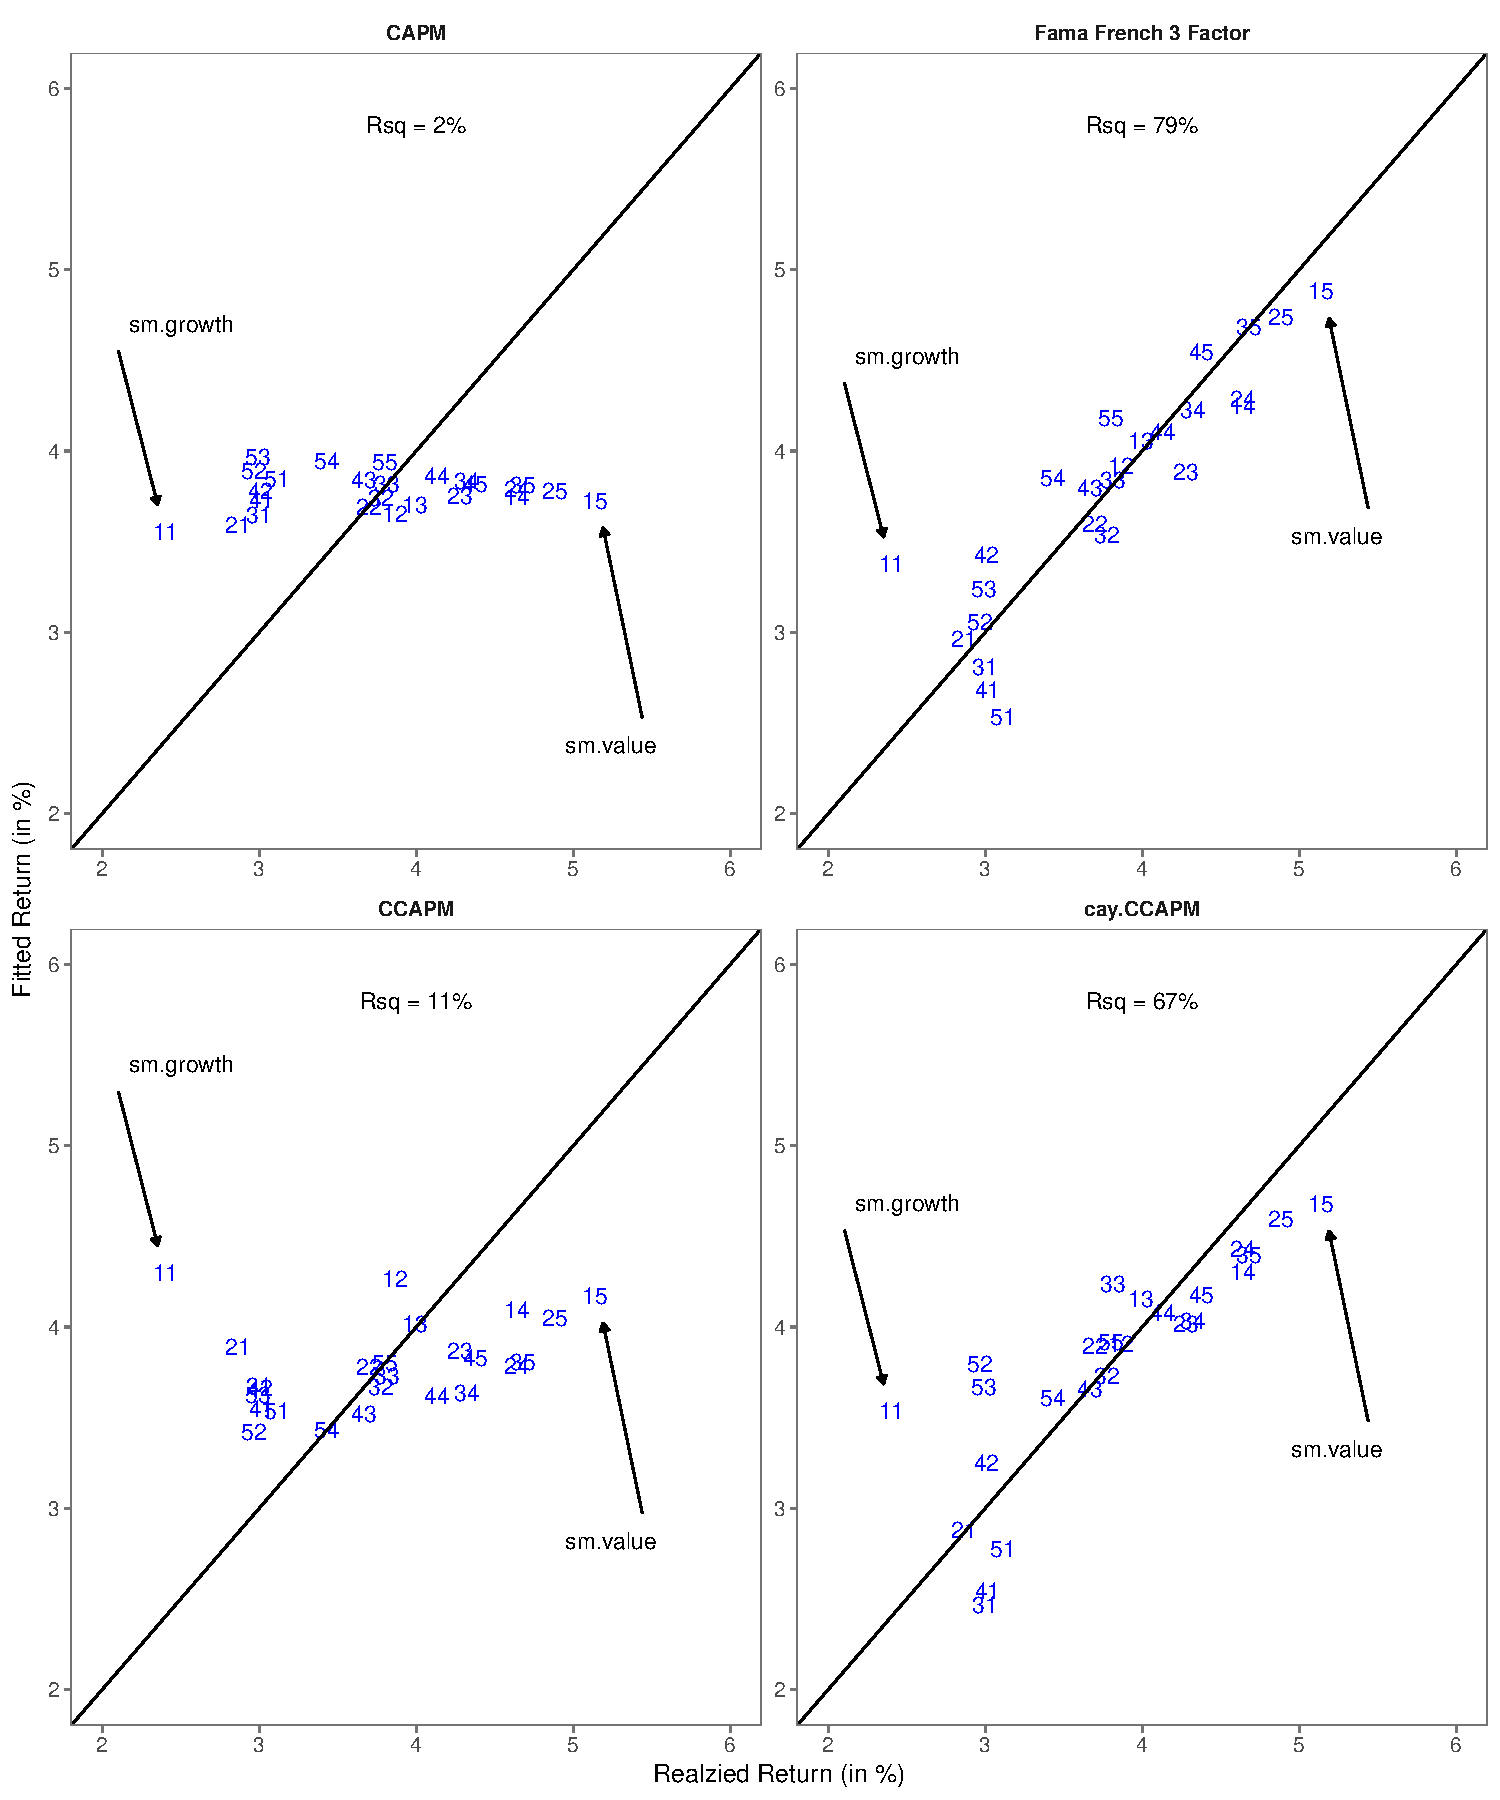
\includegraphics[scale=0.6]{fig1.pdf}
\caption{--- Realized vs. fitted returns: 25 Fama-French portfolios. The figure shows the pricing errors for each of the 25 Fama-French portfolios for the fours models. Each two-digit number represents one portfolio. The first digit refers to the size quantiles(1 indicating the smallest firms, 5 the largest), and the second digit refers to book-to-market quantiles( 1 indicating the portfolio with the lowest book-to-market ratio, 5 with the highest). The pricing errors are generated using the Fama-Macbeth regressions. The scaling variable is $\widehat{cay}_t$. The data is from \bf{1973:Q3 to 1998:Q3.} }
\label{fig:old}
\end{center}
\end{figure}

\begin{figure}[htbp]
\begin{center}
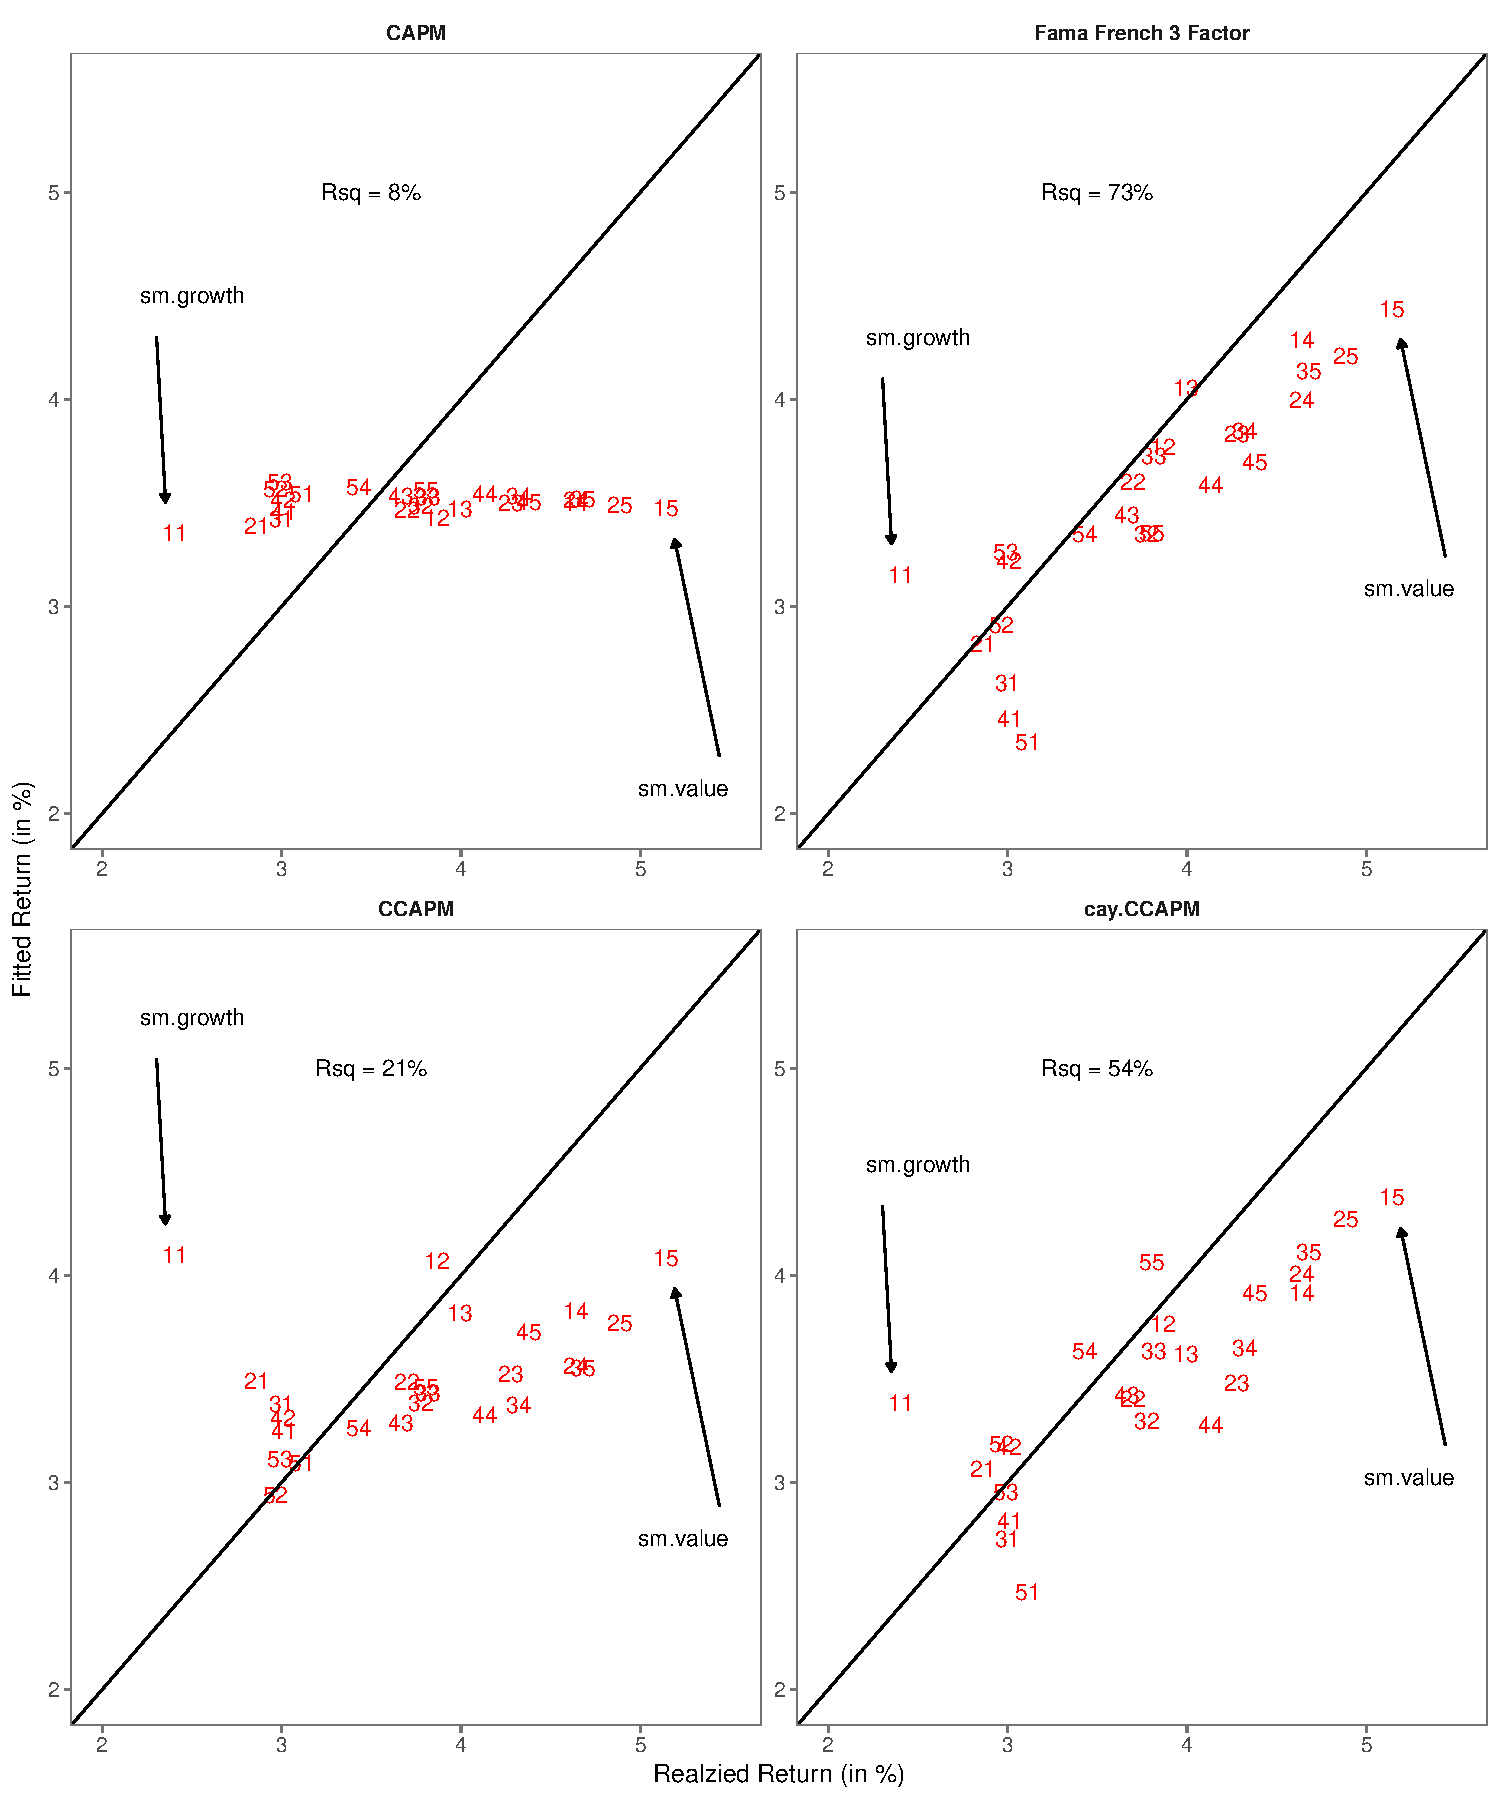
\includegraphics[scale=0.6]{fig1_full.pdf}
\caption{--- Realized vs. fitted returns: 25 Fama-French portfolios. The figure shows the pricing errors for each of the 25 Fama-French portfolios for the fours models. Each two-digit number represents one portfolio. The first digit refers to the size quantiles(1 indicating the smallest firms, 5 the largest), and the second digit refers to book-to-market quantiles( 1 indicating the portfolio with the lowest book-to-market ratio, 5 with the highest). The pricing errors are generated using the Fama-Macbeth regressions. The scaling variable is $\widehat{cay}_t$.The data is from \bf{1973:Q3 to 2015:Q3.}}
\label{fig:new}
\end{center}
\end{figure}



\begin{landscape}
\begin{threeparttable}[htbp]
\centering
\label{table:old}
\caption{  Fama-Macbeth Regressions Using 25 Fama-French Portfolios: $\lambda_j$ Coefficient Estimates on Betas in Cross-sectional Regression,  Test for Joint Significance, and Test for Zero Pricing Errors($\alpha$) with data from \textbf{1973:Q3 to 1998:Q3.} } 
\begin{tabular}{lccccccccccccc}
  \toprule
  \midrule
   & &  & \multicolumn{5}{c}{$\text{Factors}_{t+1}$}  & \multicolumn{3}{c}{$\widehat{cay}_t \cdot \text{Factors}_{t+1}$} & $R^2$ & \multirow{2}{2cm}{\centering Joint Significance} & \multirow{2}{2.5cm}{ \centering Alpha Test ($\chi^2$)} \\ \cmidrule(lr){4-8} \cmidrule(lr){9-11}
 Row & Constant & $\widehat{cay}_t$ & $R_{vw}$ & $\Delta y$ & $\Delta c$ & SMB & HML & $R_{vw}$  & $\Delta y$ & $\Delta c$ & $(\bar{R}^2)$ & & \\ \midrule
1 & 4.35 &  & -0.49 &  &  &  &  &  &  &  & 0.02 & 0.683 & 60.1 \\ 
   & (4.59) &  & (-0.41) &  &  &  &  &  &  &  & -0.02 & (0.684) & (0.000) \\ 
   & (4.28) &  & (-0.41) &  &  &  &  &  &  &  &  &  &  \\ 
  2 & 3.28 &  &  &  & 0.2 &  &  &  &  &  & 0.11 & 0.288 & 52.61 \\ 
   & (5.07) &  &  &  & (1.06) &  &  &  &  &  & 0.07 & (0.367) & (0.001) \\ 
   & (4.66) &  &  &  & (0.98) &  &  &  &  &  &  &  &  \\ 
  3 & 2.02 &  & 1.19 &  &  & 0.43 & 1.51 &  &  &  & 0.79 & 0.002 & 41.958 \\ 
   & (1.51) &  & (0.78) &  &  & (0.85) & (3.35) &  &  &  & 0.76 & (0.005) & (0.006) \\ 
   & (1.49) &  & (0.77) &  &  & (0.85) & (3.22) &  &  &  &  &  &  \\ 
  4 & 4.82 & 0 & -1.41 & 0.014 &  &  &  & 0.04 & 7e-05 &  & 0.62 & 0.009 & 11.961 \\ 
   & (5.02) & (-0.95) & (-1.2) & (2.21) &  &  &  & (1.74) & (2.06) &  & 0.52 & (0.159) & (0.917) \\ 
   & (4.62) & (-0.93) & (-1.18) & (1.19) &  &  &  & (1.61) & (1.71) &  &  &  &  \\ 
  5 & 4.52 & 0 &  &  & 0.01 &  &  &  &  & 0.01 & 0.67 & 0.002 & 27.48 \\ 
   & (6.24) & (-0.62) &  &  & (0.07) &  &  &  &  & (2.98) & 0.63 & (0.081) & (0.194) \\ 
   & (5.52) & (-0.61) &  &  & (0.07) &  &  &  &  & (2.39) &  &  &  \\ 
\bottomrule
\end{tabular}
\begin{tablenotes}\footnotesize
 \item \quad Note. The table presents $\bm{\lambda}$ (risk prices) estimates from cross-sectional Fama-Macbeth regressions using returns of 25 Fama-French portfolios: $\E[R_{i,t+1}] = \E[R_{0,t}] + \bm{\beta}^{\prime} \bm{\lambda} $. The individual $\lambda_j$ estimates for the beta of the factor listed in the column heading are reported. The scaling variable is $\widehat{cay}_t$. The table reports the Fama-Macbeth cross-sectional regression coefficient; in parentheses are two  $t$-statistics for each coefficient estimate. The top statistic uses uncorrected Fama-Macbeth standard errors; the bottom statistic uses the Shanken(1992b) correction. The term $R^2$ denotes the unadjusted Jaganathan-Wang(1996) $R^2$, and $\bar{R}^2$ adjusts for the degrees of freedom. The column Joint Significance presents $p$-values from $\chi^2$ tests of joint significance for all the right-hand-side betas. The top number is computed using the uncorrected variance-covariance matrix, and the bottom number in parenthesis uses the Shanken(1992b) correction. The column Alpha Test reports the $\chi^2$ statistic for a cross-sectional test that the pricing error is zero, the bottom number in parenthesis is the corresponding $p$-values for the alpha test. 
 \item \quad The model is estimated using data from 1973:Q3 to 1998:Q3. 
%\item \quad $*$ Statistically different from zero at the 5 percent level.
\end{tablenotes}
%\raggedright
\end{threeparttable}
\end{landscape}






\begin{landscape}
\begin{threeparttable}[htbp]
\centering
\label{table:new}
\caption{  Fama-Macbeth Regressions Using 25 Fama-French Portfolios: $\lambda_j$ Coefficient Estimates on Betas in Cross-sectional Regression,  Test for Joint Significance, and Test for Zero Pricing Errors($\alpha$) with data from \textbf{1973:Q3 to 2015:Q3. }} 
\begin{tabular}{lccccccccccccc}
  \hline
  \hline
   & &  & \multicolumn{5}{c}{$\text{Factors}_{t+1}$}  & \multicolumn{3}{c}{$\widehat{cay}_t \cdot \text{Factors}_{t+1}$} & $R^2$ & \multirow{2}{2cm}{Joint Significance} & \multirow{2}{*}{Alpha Test } \\ \cmidrule(lr){4-8} \cmidrule(lr){9-11}
 Row & Constant & $\widehat{cay}_t$ & $R_{vw}$ & $\Delta y$ & $\Delta c$ & SMB & HML & $R_{vw}$  & $\Delta y$ & $\Delta c$ & $(\bar{R}^2)$ & & \\ \midrule
1 & 3.84 &  & -0.3 &  &  &  &  &  &  &  & 0.01 & 0.779 & 85.339 \\ 
   & (4.18) &  & (-0.28) &  &  &  &  &  &  &  & (-0.04) & (0.779) & (0.000) \\ 
   & (4.02) &  & (-0.28) &  &  &  &  &  &  &  &  &  &  \\ 
  2 & 2.7 &  &  &  & 0.32 &  &  &  &  &  & 0.21 & 0.091 & 72.948 \\ 
   & (4.88) &  &  &  & (1.69) &  &  &  &  &  & (0.18) & (0.166) & (0.000) \\ 
   & (4.62) &  &  &  & (1.53) &  &  &  &  &  &  &  &  \\ 
  3 & 4.82 &  & -1.96 &  &  & 0.61 & 1.14 &  &  &  & 0.73 & 0.002 & 61.193 \\ 
   & (5.34) &  & (-1.83) &  &  & (1.56) & (2.78) &  &  &  & (0.69) & (0.003) & (0.000) \\ 
   & (5.01) &  & (-1.78) &  &  & (1.55) & (2.72) &  &  &  &  &  &  \\ 
  4 & 5.67 & -0.01 & -2.81 & -0.004 &  &  &  & -0.16 & 8e-05 &  & 0.67 & 0.002 & 29.549 \\ 
   & (4.81) & (-1.44) & (-2.15) & (-1.86) &  &  &  & (-3.23) & (1.03) &  & (0.58) & (0.117) & (0.078) \\ 
   & (4.56) & (-1.25) & (-2.05) & (-1.7) &  &  &  & (-2.36) & (0.96) &  &  &  &  \\ 
  5 & 2.93 & 0.01 &  &  & 0.23 &  &  &  &  & 0.02 & 0.54 & 0.005 & 31.204 \\ 
   & (3.75) & (1.16) &  &  & (1.12) &  &  &  &  & (2.39) & (0.47) & (0.277) & (0.092) \\ 
   & (3.63) & (1.08) &  &  & (1.07) &  &  &  &  & (1.57) &  &  &  \\ 
\bottomrule
\end{tabular}
\begin{tablenotes}\footnotesize
 \item \quad Note. The table presents $\bm{\lambda}$ (risk prices) estimates from cross-sectional Fama-Macbeth regressions using returns of 25 Fama-French portfolios: $\E[R_{i,t+1}] = \E[R_{0,t}] + \bm{\beta}^{\prime} \bm{\lambda} $. The individual $\lambda_j$ estimates for the beta of the factor listed in the column heading are reported. The scaling variable is $\widehat{cay}_t$. The table reports the Fama-Macbeth cross-sectional regression coefficient; in parentheses are two  $t$-statistics for each coefficient estimate. The top statistic uses uncorrected Fama-Macbeth standard errors; the bottom statistic uses the Shanken(1992b) correction. The term $R^2$ denotes the unadjusted Jaganathan-Wang(1996) $R^2$, and $\bar{R}^2$ adjusts for the degrees of freedom. The column Joint Significance presents $p$-values from $\chi^2$ tests of joint significance for all the right-hand-side betas. The top number is computed using the uncorrected variance-covariance matrix, and the bottom number in parenthesis uses the Shanken(1992b) correction. The column Alpha Test reports the $\chi^2$ statistic for a cross-sectional test that the pricing error is zero, the bottom number in parenthesis is the corresponding $p$-values for the alpha test. 
 \item \quad The model is estiamted using data from 1973:Q3 to 2015:Q3. 
%\item \quad $*$ Statistically different from zero at the 5 percent level.
\end{tablenotes}
\end{threeparttable}
\end{landscape}




%%%%%%%%%%%%%%%%%%%%%%%%%
\section{Discussion}
The figure and tables shoud be self-explanatory, here are some additional comments.
\begin{enumerate}
 \item Table \ref{table:old} is comparable to the original data only for some minor difference in values. The noticeable difference is for row 4, which is the CAPM with human capital scaled with cay, the $R^2$ is only $62\%$ compared to the original paper's number of $77\%$, this is due to the labor income growth I used is different from Jaganathan and Wang. \footnote{I contact the author but he no longer has the data, it was accessible through an anonymous FTP back to the time the original paper was written }
 \item  The goodness of fit for Fama French 3 Factor and cay scaled CCAPM decrease with extended data while the $R^2$ increase for CCAPM and CAPM with human capital scaled with cay. This means the preferred models in the original paper are no longer good enough to explain the asset returns behaviors. This is mostly easily seen in figure \ref{fig:new} for Fama French 3 Factor and cay scaled CCAPM models, the portfolios are generally below the 45 degree line, the realized return are too large to be explained by the models. This implies that there are certain risk factors missing from the current model, which account for the pricing errors. \footnote{From 2015, Martin Lettau and Sydney Ludvigson suggested to using a Markov Switching cay, I used the MS-cay from Martin Lettau's website, there's no material difference from the current results.}
 Meanwhile, the consumption CAPM with extended data starts to line up with the 45 degree line better, labor income growth rate help to explain asset returns better than Fama French 3 factor, these suggest that macroeconomic factors are proper factors to consider for asset pricing in the long term.
 \item Fama Macbeth impose the assumption that errors are independent over time, hence it only controls for cross-sectional correlation, and simply use time-series average to estimate the values of $\lambda$ coefficients and relevant variance-covariance matrix for cross-sectional errors and $\bm{\lambda}$ vector. However, I found strong time-series cross-correlation between factors (this shouldn't be surprising especially for macroeconomic factors), this means that Fama-Macbeth procedure under-estiamtes the true variance-covariance matrix for cross-sectional errors and $\bm{\lambda}$ vector. Although Shanken's correction is designed to correct it, it also assumes that the model is correctly specified, hence it turns out to be too small with my exploration. \footnote{There are two ways to estimate the variance-covariance matrix $\bm{\lambda}$ vector, they are quite different for some of the models including Fama-French 3 factor model, one of them has the null that the model is correctly specified to correct for cross-sectional correlation among errors, this was not the case since many of the estimated variance-covariance matrix for cross-sectional errors are computationally singular from my finding.}
 \item The GMM is not used because the preferred weighting matrix is Identity matrix, which is numerically the same as Fama-Macbeth regression, because panel data with Identity matrix in GMM is just pooled OLS which assumes i.i.d cross-sectional variance-covariance matrix over time. Alternative weighting matrix will price combinations of Fama-French 25 portfolios, which undo the task of trying to find factors that price exactly the cross-sectional variation of the 25 portfolios. \footnote{As pointed out in Ludvigson's NBER summer institute class.}
\item The joint alpha test is unreliable in small sample and the current research.
\begin{enumerate}[label=(\alph*)]
 \item The joint alpha test, or the zero pricing error test has bad property in small samples, as acknowledged by the authors themselves, therefore we should be conservative towards the test result. In particular, cay scaled models has a smaller Chi-square test statistics because the larger time series variation of macroeconomic variables leads to a bigger Shanken's correction.
\item The variance-covariance matrices are underestimated in small samples, this is because Fama-Macbeth impose time series independence and simply use time series average as estimates. 
\item I found strong cross-sectional correlations, the variance-covariance matrix are computationally singular, and are ill-conditioned. This makes the chisquare statistics very unreliable because the machine number inaccuracy will blow up. ?The test requires the inverse of variance-covariance matrix)
\item The cross-sectional error corrections are done with estimation of betas in the Fama Macbeth procedure. With small sample the estimation for betas ate likely to be imprecise and fail to correct the cross sectional errors, leading to ill posed matrix.
\item I conduct a block bootstrapped exercise for the Fama-Macbeth generated alpha test $\chi^2$ statistic using data for Fama-French 3 factors. The result is presented in figure \ref{fig:boot}. If Fama-Macbeth's assumption of time-series independent errors is correct, the bootstrapped density should be similar to that theoretical $\chi^2$ distribution. It's obvious the bootstrapped  density shifts to the right, reflects a variance-covariance estimate too small.
\end{enumerate}
\begin{figure}[htbp]
\begin{center}
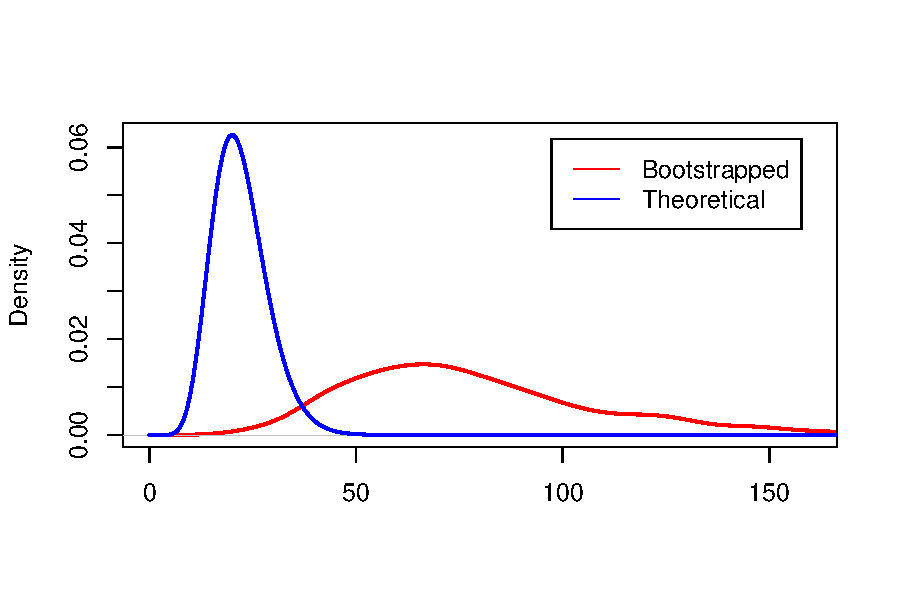
\includegraphics[scale=0.81]{bootstrap.pdf}
\caption{Theoretical v.s bootstrapped density for $\chi^2$ test statistic for zero pricing errors with data for Fama-French 3 factor model. The sample data are block bootstrapped with block size of 8 quarters.}
\label{fig:boot}
\end{center}
\end{figure}


\end{enumerate}


%%%%%%%%%%%%%%%%%%%%%%%%%%%%%%%%

\end{document}

%%%%%Matrix
%\begin{bmatrix}
%    x_{11} & x_{12} & x_{13} & \dots  & x_{1n} \\
%    x_{21} & x_{22} & x_{23} & \dots  & x_{2n} \\
%    \vdots & \vdots & \vdots & \ddots & \vdots \\
%    x_{d1} & x_{d2} & x_{d3} & \dots  & x_{dn}
%\end{bmatrix}
%\]
